


\begin{center}
  \begin{minipage}{0.6\textwidth}
    \textsl{Ce qui suit n'est pas propre à Linux, ni à Unix, bien sûr.
      La deuxième partie (commandes Linux, page \pageref{netlinux}),
      elle, est spécifique à Unix 
      (Linux).} 
  \end{minipage}
\end{center}
\section{Réseau: le modèle en couches de l'Open Systems Interconnection
  (OSI}
L'idée est comme souvent en informatique de  cacher de l'information:
la couche de niveau $n$ du réseau n'a pas à savoir comment fonctionne la  couche
de niveau $n-1$, comment elle 
assure son service (voir \cite{OSI}). Ce qui va nous 
intéresser apparaît au niveaux 3 et 4; les niveaux 1 et 2 sont
chargés des aspects matériels du réseau. Notez que, dans ce modèle,
on peut changer la réalisation pratique d'un niveau sans que les
niveaux supérieurs en soient affectés.

Ce qui va nous intéresser:
\begin{itemize}
  \item Le niveau 3: Internet Protocol, avec deux versions, IPv4 et
    IPv6. Ce niveau propage des paquets d'information, de taille bornée.
  \item Le niveau 4. Les paquets du niveau 3 transportent les données
    utiles.  Les
    données transportées sont d'un type donné, spécialement:
    \begin{itemize}
      \item ICMP  (Internet Control Message Protocol): transmission de
        messages à usage interne du réseau (messages d'erreur, echo,
        etc.)\cite{icmp}.
      \item UDP et TCP: UDP\cite{udp} est un protocole
        \emph{léger}: peu de 
        contrôles, pas d'accusé de réception à la différence de TCP\cite{tcp}.
    \end{itemize}
    A ce niveau, on définit aussi la notion de \emph{port}, étiquetés
    par des numéros et associés à des services ou des applications.

    Les paquets de données sont transportés sans connexion, c'est à
    dire que les données qu'ils contiennent sont suffisantes pour
    assurer leur livraison, sans qu'une connexion figée soit établie;
    on parle de \emph{datagramme}\cite{dgram}. Un des inventeurs de la
    notion de datagramme est Louis
    Pouzin\cite{pouzin}\footnote{Intervenant aux JDLL il y a quelques années.}. 
\end{itemize}
\section{Réseau, configuration classique: machines derrière une \og
  box\fg}

\begin{figure}
  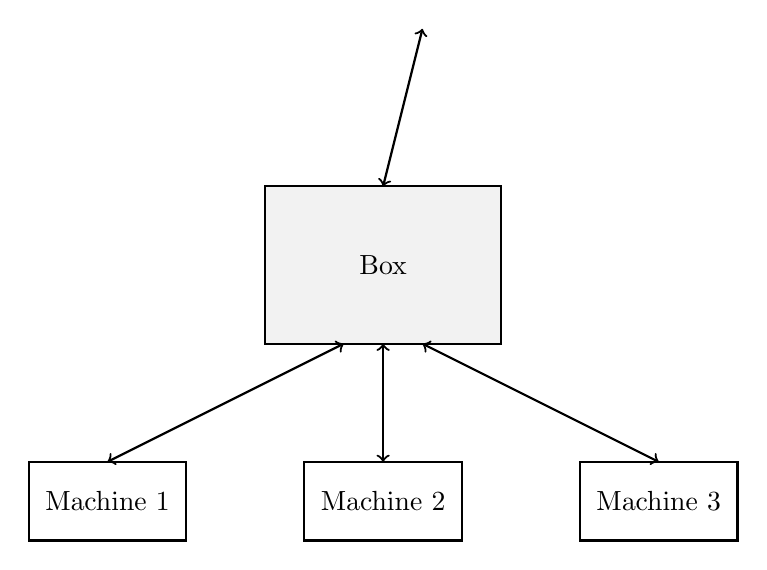
\begin{tikzpicture}[level distance=10mm,thick]
    \draw (3,5) rectangle +(3,2) [fill=gray!10]  node[midway]
          {Box};
          
          \draw[<->] (4.5,7)--(5,9);

    \draw (0,2.5) rectangle +(2,1)  node[midway]
          {Machine 1};
          \draw[<->] (1.,3.5)--(4,5);
          
    \draw (3.5,2.5) rectangle +(2,1)  node[midway]
          {Machine 2};
          \draw[<->] (4.5,3.5)--(4.5,5);
          
    \draw (7,2.5) rectangle +(2,1)  node[midway]
          {Machine 3};
          \draw[<->] (8,3.5)--(5,5);
    
  \end{tikzpicture}
  \caption{machines derrière une  \og   box\fg}\label{box}
\end{figure}

\subsection{Le cas \og classique\fg{}: IPv4}
Toute machine a une adresse, qui en IPv4 ressemble à
134.214.100.121 et chaque adresse est unique sur l'internet. Les 4 nombres 
qui forment l'adresse sont stockés chacun sur un octet ce qui
correspond à des nombres compris entre $0$ et $255$
(bornes incluses)\footnote{Car $255 = 1+2 +4+\ldots+2^7 = 2^8 -1$.}. L'adresse
IPv4 est donc stockée sur 4 octets (soit 32 bits)  et le nombre d'adresses
disponibles est donc de $2^{32} -1= 4294967295$ soit un peu plus de 4
milliards d'adresses. Sachant que, comme on va le voir, certaines
adresses sont réservées à des usages particuliers, c'est peu et
actuellement insuffisant. IPv4 peut donc être considéré comme un
protocole en fin de vie.

La technique utilisée derrière les  \og   box\fg{} est celle du
\emph{réseau local} (voir figure \ref{box}): seule la  \og   box\fg{}
est visible du monde extérieur, possède une adresse ip connue de
l'internet. C'est ce qui a permis à IPv4 de survivre jusqu'à
aujourd'hui, car cela permet de cacher des machines à l'internet.  La
\og   box\fg{} a des interfaces sur deux réseaux: le 
réseau local, et le réseau extérieur.
\subsubsection{Le réseau local:}

\begin{itemize}
  \item les machines du sous réseau local: elles  ont des adresses
    dont les deux octets de gauche sont
  192.168. Ces adresses ne sont certainement pas
  uniques, mais sont invisibles de l'internet. La \og box\fg{} agit
    comme un barrage, laissant quand même passer (on va voir comment)
    ce qui est nécessaire. 

\end{itemize}
Cela pose un certain nombre de questions:
\begin{enumerate}

\item Comment sont affectées
  les adresses aux machines du réseau local? à ma \og box\fg?
\item Comment les machines du réseau local
  communiquent-elles avec le mode extérieur?
\item Comment fait-on, depuis une machine du réseau local,  pour
  joindre une machine extérieure au réseau 
  local, connaissant son nom?
\end{enumerate}

Et bien sûr quels sont les outils Linux (Unix) associés, quelles sont
les commandes qui permettent d'explorer ce fonctionnement?

Auparavant il faut comprendre un peu comment fonctionne IP (v4 dans ce
cas).
\subsection{Internet protocol}
Un paquet IP est formé d'une en-tête et de données. L'en-tête pour
IPv4 est
décrite à la figure \ref{entetev4}. Pour une description détaillée,
consulter par exemple \cite{v4}. Parmi les champs de l'en-tête,
retenons:
\begin{itemize}
  \item L'adresse source:
    adresse IP de l'émetteur.
  \item L'adresse du destinataire.
  \item Le protocole (8 bits):
    numéro du protocole au-dessus de la couche réseau : TCP = 6, UDP =
    17, ICMP = 1.
   \item Identification (16 bits):
    Numéro permettant d'identifier les fragments d'un même paquet.
\end{itemize}
\begin{figure}
  \includegraphics[width=0.8\textwidth]{images/entetev4.png}
  \caption{En-tête IPv4}\label{entetev4}
\end{figure}
\subsection{Le NAT (Network Adress Translation}\label{nat}
Supposons que la machine 1 (figure \ref{box}) veuille envoyer un
paquet à l'extérieur. La box (un système Linux, à priori) va changer
l'adresse ip  de la machine 1 par sa propre adresse, et se
souvenir d'un identifiant unique du paquet. Au retour, il enverra le
paquet de retour vers la machine 1 (c'est un peu simplifié). Donc, de
l'extérieur, on ne voit que la \og box\fg\footnote{Le NAT est une
  fonctionalité du noyau Linux. Voir page \pageref{firewall}.}

Comment tester ça? Il suffit d'aller sur le site
\url{https://www.whatismyip.com/fr/}: si vous avez plusieurs machines
dans votre réseau local (ordinateur, téléphone sur le wi-fi, etc.)
quelque soit la machine que vous utiliserez pour consulter cette url,
vous obtiendrez la même adresse v4 (à condition bien sûr que vous
soyez encore sur un réseau IPv4).

Bien, mais ceci ne nous dit pas:
\begin{enumerate}
\item Comment chaque machine du réseau local est configurée?
  Comment  connaît-elle les
    paramètres nécessaires à son fonctionnement (entre autres son adresse ip)?
  \item Comment la box sait-elle faire la différence entre un trafic
    local et un accès vers l'extérieur?
  \item Comment associer un nom (exemple: \ttt{www.aldil.org}) à une
    adresse ip et vice versa?
\end{enumerate}


\subsubsection{La configuration réseau d'une machine locale}
Jadis, on faisait ça à la main en remplissant un fichier. Pas très
facile, ni pratique pour un portable appelé à changer de réseau!

C'est un service: une machine dans le réseau (dans notre cas c'est la
box, mais ce peut être une autre) fait tourner un démon \ttt{DHCP}.
De façon sommaire: la machine en manque de configuration (quand elle
boote par exemple) envoie un
paquet IP en \emph{broadcast} (à la cantonade!): dans ce cas l'adresse
du destinataire  est $255.255.255.255$. Le 
paquet contient 
entre autres l'\emph{adresse MAC} (voir ci-dessous) de la machine
\emph{cliente}. Le 
serveur \ttt{DHCP} envoie alors tous les renseignements nécessaires à
la configuration réseau de la machine cliente, dont son adresse IP. Il 
se base sur l'adresse MAC, pour lui associer une adresse
IP\footnote{Plusieurs méthodes sont possibles: table faisant
  correspondre adresse MAC et adresse (l'adresse de la machine est
  alors fixe), ou tirage 
  aléatoire.}; il envoie aussi tous les autres paramètres dont la
machine a ou peut avoir besoin
(voir \cite{dhcp} pour une explication un peu détaillée). Les
renseignements envoyés par le serveur ont une durée de 
vie, qui peut être limitée ou infinie: quand les renseignements sont
périmés, la 
machine cliente refait une requête au serveur DHCP.
\subsubsection{l'adresse MAC} est un identifiant d'une
interface réseau: c'est attribué à la construction physique de la
machine, et c'est à priori 
unique. Exemple:

\begin{center}
\ttt{d8:50:e6:ba:2e:d8}
\end{center}

\subsubsection{Que faire des paquets qui ne sont pas destinés à une
  machine locale?} Il faut les envoyer à une machine qui fait office
de porte de sortie (GATEWAY). La machine du réseau local doit donc
connaître l'adresse IP de cette porte (ça fait partie des paramètres
renvoyés par le serveur DHCP). La machine GATEWAY a deux interfaces
réseau configurées, et donc deux adresses IP:
\begin{enumerate}
  \item une sur le réseau local (celle que connaissent les machines du
    réseau local),
  \item une adresse sur le réseau extérieur (celui du FAI dans notre
    cas). C'est celle qu'on voit quand on va sur le site
    \url{https://www.whatismyip.com/fr/}.
\end{enumerate}
Dans notre cas, la GATEWAY  c'est la box, mais ce n'est
pas obligatoire.
\subsubsection{Netmask (masque de sous-réseau)}
Supposons que mon adresse ip soit 51.75.22.226. Quelles sont les
adresses qui font partie du même sous-réseau que moi? Le sous-réseau
peut être mon réseau local privé derrière ma box, ou, disons le réseau
free.fr ou...?

La règle est que les  adresses d'un même sous-réseau partagent un
début d'adresse (partie 
gauche) commune. On trouve en général la notation
192.168.0.10/24. Dans ce cas cela veut dire que les 24 premiers bits
en partant de la gauche sont communs aux adresses du réseau. Ici $24 =
3 \times 8$ et donc les adresses de l'ensemble des machines  du
réseau (local) sont de la
forme 192.168.0.*. Le masque donne donc aussi la taille du
sous-réseau (254 adresses ici\footnote{La valeur 255 est réservée
  comme on le verra plus bas.}).

Toujours dans l'exemple ci-dessus, le nombre de 4 octets ayant 24 de ses
bits de gauche à 1 et les autres à 0 s'écrit (en base 2 et en séparant
les octets par un ``.''): 

$$11111111.11111111.11111111.00000000$$

et comme $11111111 = 255$ en base 10, cela peut se noter:

$$255.255.255.0$$

qui est le \emph{netmask} du réseau.

Cela permet de répondre à la question suivante: étant donné une
adresse IPv4, est-elle dans le même réseau que moi? Là, il faut faire
un peu de logique: on assimile 0 à la valeur \emph{faux} et 1 à la
valeur \emph{vrai}\footnote{Vous pouvez aussi voir ça comme une
  multiplication, remplacer ET par $\times$.}. On a: 

\begin{itemize}
\item 0 ET 0 = 0 (faux et faux est faux)
\item 0 ET 1 = 0 (faux et vrai est vrai)
\item 1 ET 0 = 0 (vrai et faux est faux)
\item 1 ET 1 = 1 (vrai et vrai est vrai).
\end{itemize}


 On fait un \og ET\fg{} bit à bit entre le netmask et l'adresse
 testée.

 Exemples:
 \begin{itemize}
 \item Considérons l'adressse \ttt{192.168.0.21}, le netmask étant
 \ttt{255.255.255.0}. 

   \ttt{192.168.0.21} est \ttt{11000000.10101000.00000000.00010101} en
   binaire.

   Le netmask est \ttt{11111111.11111111.11111111.0000000}.

   Le ``ET''
   entre le netmask et mon adresse ip est:

   \begin{center}
     \begin{minipage}{0.44\textwidth}
       \begin{flushleft}
\begin{verbatim}
11000000.10101000.00000000.00010101
11111111.11111111.11111111.00000000
\end{verbatim}
\rule{\textwidth}{.1pt}
\begin{verbatim}
11000000.10101000.00000000.00000000
\end{verbatim}
     \end{flushleft}
     \end{minipage}
   \end{center}

  Le résultat,  \ttt{11000000.10101000.00000000.00000000}, est $192.168.0.0$ en
   base 10.
   
   
 \item Pour l'adresse 192.168.0.32, le calcul précédent donne le même
   résultat: les deux adresses sont donc dans le même réseau.
 \item Mais pour 134.214.100.8, le résultat est différent, et les deux
   adresses ne sont donc pas dans le même réseau.
\end{itemize}
   
 

\subsubsection{Adresse de broadcast}
Comment contacter toutes les machines du même réseau?

On considère la partie commune des adresses du réseau: dans mon cas,
utilisant le netmask 255.255.255.0, et mon adresse étant 192.168.0.32,
j'en déduis que les machines de mon réseau ont toutes des adresses de
la forme 192.168.0.x ou x est compris entre 0 et 255. L'adresse de
broadcast est obtenue en remplaçant ``x'' par 255 (soit  des 1 partout
en binaire), ce qui
ici donne:

$$192.168.0.255.$$

Envoyer un paquet IP avec cette adresse de destinataire, c'est écrire
à toutes les machines du réseau.

Noter que:
\begin{itemize}
  \item L'adresse 192.168.0.255 est réservée pour le \emph{broadcast}:
    elle ne peut donc pas être affectée à une machine particulière et,
    dans le cas envisagé ici, il ne peut y avoir que 254 machines dans
    notre réseau local.
  \item On a déjà  vu un \emph{broadcast} à propos du DHCP, où
    l'adresse était $255.255.255.255$ pour le \emph{broadcast} . Ce n'est
    pas exactement la même chose.
\end{itemize}
\subsubsection{Serveur de noms (DNS, Domain Name System)}
La configuration réseau d'une machine contient au minimum 4
paramètres:
\begin{enumerate}
\item l'adresse IP,
\item le netmask,
\item l'adresse de la GATEWAY,
\item et l'adresse du \emph{serveur de noms.}
\end{enumerate}
Le \emph{serveur de noms} est chargé d'associer un nom
(\ttt{www.aldil.org} par exemple) à une adresse ip, et vice-versa.

Supposons que je cherche l'adresse de \ttt{math.univ-lyon1.fr}; le
fonctionnement est à peu près le suivant: 
\begin{enumerate}
  \item Est-ce que ma machine connaît l'adresse IP de
    \ttt{math.univ-lyon1.fr}? Si oui, c'est fini. Sinon, ma machine envoie une
    requête au serveur de noms précédemment défini (par la
    configuration de ma machine --obtenue par le serveur DHCP de mon réseau--).
  \item Est ce que ce serveur de noms connaît l'adresse que je cherche?
    Dans mon cas le serveur de nom peut être un serveur qui tourne
    dans la box, ou bien  celui de mon FAI, disons
    \ttt{free.fr}. Si le serveur a la réponse, c'est fini, sinon, il
    faut monter d'un cran.
  \item Si le serveur de noms de \ttt{free.fr} connaît l'adresse du
    serveur de nom de \ttt{univ-lyon1.fr}, il lui demande l'adresse de
    \ttt{math.univ-lyon1.fr}; peut être faut-il une étape
    supplémentaire si  \ttt{univ-lyon1.fr} est inconnu chez
    \ttt{free.fr}: dans ce cas il consulte le DNS de \ttt{fr}, qui
    connaît \emph{obligatoirement} \ttt{univ-lyon1.fr}.
  \item  Le serveur de noms de \ttt{univ-lyon1.fr} connaît
    \emph{obligatoirement} l'adresse cherchée (ainsi que les adresses de
    toutes les machines du domaine \ttt{univ-lyon1.fr}: c'est stocké
    dans des tables).
  \item Une fois un serveur capable de répondre à notre requête
    atteint, celui envoie l'adresse IP, mais aussi une durée garantie
    de validité de cette adresse. Alors \emph{tous} les serveurs de noms
    et au bout votre machine elle-même vont se souvenir de ce
    renseignement, pendant un temps fixé, ce
    qui  permet de limiter le trafic sur le réseau\footnote{C'est très
      utile quand on envisage de changer des adresses: on diminue la
      durée de validité.}.
    
\end{enumerate}
Évidemment les serveurs DNS contenant des tables associant adresses
et noms, la recherche fonctionne en sens inverse: connaîssant l'adresse
ip, trouver le nom. 
\subsection{En résumé}
Pour IPv4, il faut au minimum  4 paramètres pour définir la
configuration réseau d'une machine:
\begin{itemize}
\item L'adresse de la machine.
\item Celle de la GATEWAY.
\item Celle du DNS.
\item Le netmask.
\end{itemize}
Pour une description plus détaillée consulter par exemple \cite{dns}.

\subsection{IPv6}
  Les adresses ne sont plus stockées sur 32 bits mais sur 128 bits (16
  octets).

  Petit calcul:

  \begin{itemize}
    \item le rayon $R$ de la terre est de 6000 kms environ, soit $6000
      \times 1000$ mètres. la surface de la terre est  donc environ (en
      mètres carrés) de
      $$S= 4 \pi R^2.$$
    \item Le nombre d'adresses IP v6 disponibles par mètre carré est
      donc environ:
      $$\frac{2^{128}-1 }{4 \pi R^2},$$
      ce qui fait environ $7,5\times  10^{23}$ adresses au mètre
          carré\footnote{Comment je calcule ça? Avec SageMath:
            \url{https://www.sagemath.org/} et
            \url{http://sagebook.gforge.inria.fr/english.html}.
          Notons que $10^{23}$ c'est 100 000 miliards de milliards.}!
  \end{itemize}

  La notation des adresses est un peu différente. Cela pourra être:

  \begin{center}
  \ttt{2001:0db8:0000:85a3:0000:0000:ac1f:8001}
  \end{center}
  
  Pourquoi des lettres (\ttt{d}, \texttt{b}, \ttt{a})? Ces  adresses
  sont écrites 
  en base 16 pour laquelle on note les chiffres
  $0,1,\ldots,9,a,b,c,d,e,f$ (15 chiffres), ce qui rend l'écriture plus
  compacte. Des écritures condensées existent, voir \cite{v6}.

  \subsubsection{Notes importantes}
  \begin{itemize}
    \item La migration vers v6 est en cours (v6 est disponible chez
    free.fr et adopté en remplacement de v4 chez orange (peut-être
    seulement sur certaines parties du réseau?)).
    \item IPv4 et IPv6 forment deux réseaux différents qui peuvent
      communiquer par des passerelles.
    \item Il est bien évident qu'avec IPv6, le NAT disparaît. Chacune
      de vos machines, est accessible directement derrière votre
      box! (et tous les ports de toutes les machines peuvent à priori
      être accédés). Toutes vos machines sont directement sur
      l'internet, ont chacune une adresse IPv6,  mais ceci n'empêche
      pas d'avoir des adresses 
      locales, pas visibles de l'extérieur, c'est à dire correspondant à
      votre réseau privé.
    \item Pour le netmask, rien de changé, on adapte juste à la
      longueur de l'adresse.
    \item Le DNS est adapté.
    \item Si vous êtes sur un réseau en IPv6 (vous pouvez être sur les
      deux: v4 et v6), vous pourrez vérifier en allant sur
      \url{https://www.whatismyip.com/fr/} que des machines
      différentes ont des adresses IPv6 différentes, même derrière
      votre box. Mais il se peut aussi que certaines machines de votre
      réseau (c'est le cas de mon téléphone connecté au wifi de ma
      box) ne soient pas configurées pour se connecter en IPv6.
  \end{itemize}

\subsection{Ports} A chaque adresse IP (v4 ou v6) on associe des ports, qui sont
des nombres entiers. Cela permet de séparer le trafic. Chaque protocole
est associé à un ou plusieurs ports. Par exemple le port 80 est
associé à \ttt{http}, et un serveur web écoutera à priori sur ce port.

Dans le cas de ma box, il est possible de \emph{router} un port donné
sur vers machine du réseau local, par exemple le port 80 vers la
machine 1\footnote{Ce qui restreint les possibilités: un seul serveur
  web  dans le réseau local peut être visible de l'extérieur, par exemple.}.

    
